\documentclass[journal,12pt,twocolumn]{IEEEtran}

\usepackage[utf8]{inputenc}
\usepackage{kvmap}
\usepackage{graphics} 

\usepackage{setspace}
\usepackage{gensymb}

\singlespacing


\usepackage{amsthm}

\usepackage{mathrsfs}
\usepackage{txfonts}
\usepackage{stfloats}
\usepackage{bm}
\usepackage{cite}
\usepackage{cases}
\usepackage{subfig}

\usepackage{longtable}
\usepackage{multirow}

\usepackage{enumitem}
\usepackage{mathtools}
\usepackage{steinmetz}
\usepackage{tikz}
\usepackage{circuitikz}
\usepackage{verbatim}
\usepackage{tfrupee}
\usepackage[breaklinks=true]{hyperref}
\usepackage{graphicx}
\usepackage{tkz-euclide}
\usepackage{float}

\usetikzlibrary{calc,math}
\usepackage{listings}
    \usepackage{color}                                            %%
    \usepackage{array}                                            %%
    \usepackage{longtable}                                        %%
    \usepackage{calc}                                             %%
    \usepackage{multirow}                                         %%
    \usepackage{hhline}                                           %%
    \usepackage{ifthen}                                           %%
    \usepackage{lscape}     
\usepackage{multicol}
\usepackage{chngcntr}

\DeclareMathOperator*{\Res}{Res}

\renewcommand\thesection{\arabic{section}}
\renewcommand\thesubsection{\thesection.\arabic{subsection}}
\renewcommand\thesubsubsection{\thesubsection.\arabic{subsubsection}}

\renewcommand\thesectiondis{\arabic{section}}
\renewcommand\thesubsectiondis{\thesectiondis.\arabic{subsection}}
\renewcommand\thesubsubsectiondis{\thesubsectiondis.\arabic{subsubsection}}


\hyphenation{op-tical net-works semi-conduc-tor}
\def\inputGnumericTable{}                                 %%

\lstset{
%language=C,
frame=single, 
breaklines=true,
columns=fullflexible
}
\begin{document}


\newtheorem{theorem}{Theorem}[section]
\newtheorem{problem}{Problem}
\newtheorem{proposition}{Proposition}[section]
\newtheorem{lemma}{Lemma}[section]
\newtheorem{corollary}[theorem]{Corollary}
\newtheorem{example}{Example}[section]
\newtheorem{definition}[problem]{Definition}

\newcommand{\BEQA}{\begin{eqnarray}}
\newcommand{\EEQA}{\end{eqnarray}}
\newcommand{\define}{\stackrel{\triangle}{=}}
\newcommand\hlight[1]{\tikz[overlay, remember picture,baseline=-\the\dimexpr\fontdimen22\textfont2\relax]\node[rectangle,fill=blue!50,rounded corners,fill opacity = 0.2,draw,thick,text opacity =1] {$#1$};}
\bibliographystyle{IEEEtran}
\providecommand{\mbf}{\mathbf}
\providecommand{\pr}[1]{\ensuremath{\Pr\left(#1\right)}}
\providecommand{\qfunc}[1]{\ensuremath{Q\left(#1\right)}}
\providecommand{\sbrak}[1]{\ensuremath{{}\left[#1\right]}}
\providecommand{\lsbrak}[1]{\ensuremath{{}\left[#1\right.}}
\providecommand{\rsbrak}[1]{\ensuremath{{}\left.#1\right]}}
\providecommand{\brak}[1]{\ensuremath{\left(#1\right)}}
\providecommand{\lbrak}[1]{\ensuremath{\left(#1\right.}}
\providecommand{\rbrak}[1]{\ensuremath{\left.#1\right)}}
\providecommand{\cbrak}[1]{\ensuremath{\left\{#1\right\}}}
\providecommand{\lcbrak}[1]{\ensuremath{\left\{#1\right.}}
\providecommand{\rcbrak}[1]{\ensuremath{\left.#1\right\}}}
\theoremstyle{remark}
\newtheorem{rem}{Remark}
\newcommand{\sgn}{\mathop{\mathrm{sgn}}}
\providecommand{\abs}[1]{\left\vert#1\right\vert}
\providecommand{\res}[1]{\Res\displaylimits_{#1}} 
\providecommand{\norm}[1]{$\left\lVert#1\right\rVert$}
%\providecommand{\norm}[1]{\lVert#1\rVert}
\providecommand{\mtx}[1]{\mathbf{#1}}
\providecommand{\mean}[1]{E\left[ #1 \right]}
\providecommand{\fourier}{\overset{\mathcal{F}}{ \rightleftharpoons}}
%\providecommand{\hilbert}{\overset{\mathcal{H}}{ \rightleftharpoons}}
\providecommand{\system}{\overset{\mathcal{H}}{ \longleftrightarrow}}
	%\newcommand{\solution}[2]{\textbf{Solution:}{#1}}
\newcommand{\solution}{\noindent \textbf{Solution: }}
\newcommand{\cosec}{\,\text{cosec}\,}
\providecommand{\dec}[2]{\ensuremath{\overset{#1}{\underset{#2}{\gtrless}}}}
\newcommand{\myvec}[1]{\ensuremath{\begin{pmatrix}#1\end{pmatrix}}}
\newcommand{\mydet}[1]{\ensuremath{\begin{vmatrix}#1\end{vmatrix}}}
\numberwithin{equation}{subsection}
\makeatletter
\@addtoreset{figure}{problem}
\makeatother
\let\StandardTheFigure\thefigure
\let\vec\mathbf
\renewcommand{\thefigure}{\theproblem}
\def\putbox#1#2#3{\makebox[0in][l]{\makebox[#1][l]{}\raisebox{\baselineskip}[0in][0in]{\raisebox{#2}[0in][0in]{#3}}}}
     \def\rightbox#1{\makebox[0in][r]{#1}}
     \def\centbox#1{\makebox[0in]{#1}}
     \def\topbox#1{\raisebox{-\baselineskip}[0in][0in]{#1}}
     \def\midbox#1{\raisebox{-0.5\baselineskip}[0in][0in]{#1}}
\vspace{3cm}
\title{\textbf{Matrix Assignment - Line} }
\author{Surabhi Seetha}
\maketitle
\newpage
\bigskip
\renewcommand{\thefigure}{\theenumi}
\renewcommand{\thetable}{\theenumi}
Get Python code for the figure from 
\begin{lstlisting}
https://github.com/SurabhiSeetha/Fwciith2022/tree/main/Assignment%201/codes/src
\end{lstlisting}
Get LaTex code from
\begin{lstlisting}
https://github.com/SurabhiSeetha/Fwciith2022/tree/main/avr%20gcc
\end{lstlisting}
%
\section{Question-Class 9, Exercise 9.3, Q(1)}
\textbf{In the Figure, E is any point on median AD of a $\Delta$ ABC. Show that ar(ABE) = ar(ACE).} \\


\centering
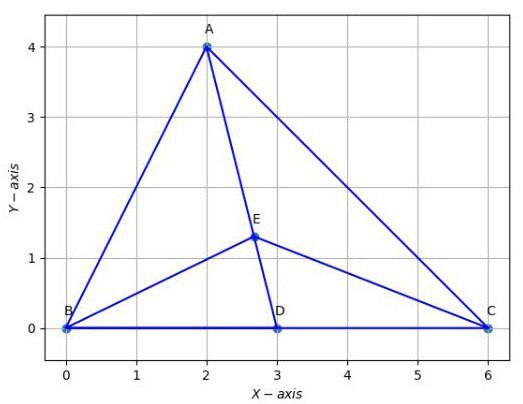
\includegraphics[width=0.45\textwidth]{Tri fig 1.jpg}
Figure 1 - Triangle ABC

\section{Construction}
\
\centering
\begin{tabular}{|c|c|c|}
\hline
\textbf{Symbol} & \textbf{Value} & \textbf{Description} \\
\hline
r & $\sqrt{20}$ & radius\\
\hline
$\theta$ & 63.45 & angle\\
\hline
B & $\begin{pmatrix} 0 \\ 0 \end{pmatrix}$ & Vertex B\\

\hline
C & $\begin{pmatrix}6 \\0 \end{pmatrix}$ & Vertex C\\
\hline

D & $\frac{B+C}{2}$ & Mid-point of BC\\
 
\hline

\end{tabular}

\centering
\begin{tabular}{|c|c|c|}

\hline

A & $\begin{pmatrix} rcos\theta \\ rsin\theta \end{pmatrix}$ & Vertex A\\

\hline

E & $\begin{pmatrix}Ex \\Ey \end{pmatrix}$ & point on AD\\

\hline

N & $\begin{pmatrix}Ax \\ 0 \end{pmatrix}$ & AN $\perp$ BC\\

\hline

M & $\begin{pmatrix}Ex \\ 0 \end{pmatrix}$ & EM $\perp$ BC\\

\hline

\end{tabular}

\section{Solution}
\raggedright{\subsection{Part-1:}}
We wish to show that
$Ar(\Delta ABE)=Ar(\Delta ACE)$\\
\vspace{0.25cm}
But to do so, firstly, we need to prove that $Ar(\Delta ABD)=Ar(\Delta ACD)$\\
\vspace{0.25cm}
Since the formula for area of a triangle is $\frac{1}{2}\times B \times H$, Let us draw an altitude $AN \perp BC$.\\
\
\begin{center}
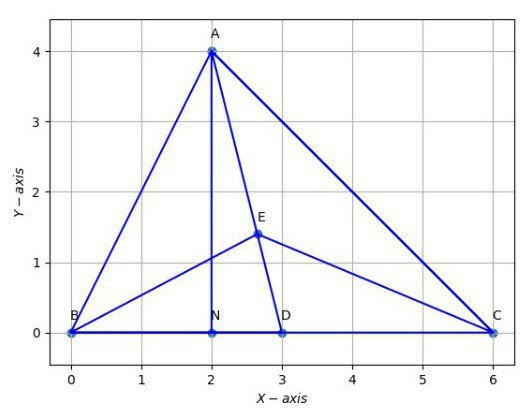
\includegraphics[width=0.4\textwidth]{Tri fig 2.jpg}\\
Figure 2 - $\Delta$ ABC with altitude ${AN} \perp {BC}$ \\
\end{center}

\hspace{0.1cm}Now, $Ar(\Delta ABD) = \frac{1}{2}$ $\times$ base $\times$ altitude of $\Delta ABD$\\
\centering
\vspace{0.25cm}
\hspace{1.6cm}$= \frac{1}{2}$ $\times$ $||{\vec{D-B}}||$ $\times$ $||{\vec{N-A}}||$\\
\vspace{0.25cm}
\
\hspace{2.9cm}\raggedright{$= \frac{1}{2}$ $\times$ $||{\vec{C-D}}||$ $\times$ $||{\vec{N-A}}||$} \vspace{0.25cm}\\
\hspace{3.5cm}{[$\because$ ${||\vec{D}-\vec{B}||}={||\vec{C}-\vec{D}||}$]}\\
\vspace{0.25cm}
\centering
\raggedright\hspace{3cm}$= \frac{1}{2}$ $\times$ base $\times$ altitude of $\Delta ACD$\\
\vspace{0.25cm}
\raggedright\hspace{2.95cm}{$=Ar(\Delta ACD)$}\\
\vspace{0.25cm}
\centering
\begin{align} 
\therefore Ar(\Delta ABD)=Ar(\Delta ACD) \hspace{0.25cm}
\label{eq:1}
\end{align}
\raggedright{\subsection{Part-2:}}

Next step is to show that $Ar(\Delta EDB)=Ar(\Delta EDC)$ by using the formula of area of a triangle.\\
\vspace{0.25cm}

To do so, now we need to draw another perpendicular from the point E onto the base $\overrightarrow{BC}$\\
\vspace{0.25cm}
\begin{center}
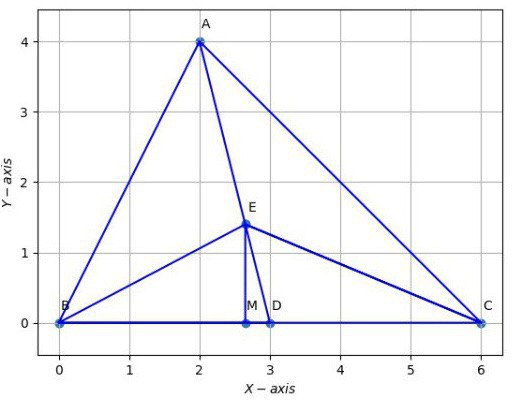
\includegraphics[width=0.4\textwidth]{Tri fig 3.jpg}\\
Figure 3 - $\Delta$ ABC with altitude ${EM} \perp {CB}$ \\
\end{center}

Now, $Ar(\Delta EDB) = \frac{1}{2}$ $\times$ base $\times$ altitude of $\Delta EDB$\\
\centering
\vspace{0.25cm}
\hspace{1.7cm}$= \frac{1}{2}$ $\times$ $||\vec{D-B}||$ $\times$ $||\vec{M-E}||$\\
\vspace{0.25cm}
\raggedright\hspace{3.0cm}{$= \frac{1}{2}$ $\times$ $||\vec{C-D}||$ $\times$ $||\vec{M-E}||$} \vspace{0.25cm}\\          
\hspace{3.5cm}{[$\because$ ${||\vec{D}-\vec{B}||}={||\vec{C}-\vec{D}||}$]}\\
\vspace{0.25cm}
\centering
\hspace{2.45cm}$= \frac{1}{2}$ $\times$ base $\times$ altitude of $\Delta EDC$\\
\vspace{0.25cm}
\raggedright\hspace{2.95cm}{$=Ar(\Delta ECD)$}\\

\centering
\begin{align}
\therefore Ar(\Delta EBD)=Ar(\Delta ECD) \hspace{0.25cm} 
\label{eqn:2}
\end{align}

\raggedright
From Fig.1, we can write that\\
\centering

\begin{align}
 Ar(\Delta ABD) = Ar(\Delta ABE) + Ar(\Delta EBD)\hspace{0.25cm} 
 \label{eqn:3}
\end{align}

\raggedright
And,
\begin{align}
Ar(\Delta ACD) = Ar(\Delta ACE) + Ar(\Delta ECD)\hspace{0.25cm} 
\label{eqn:4}
\end{align}
\raggedright
from the equation \ref{eq:1}, we can say that,
\centering
$$Ar(\Delta ABD)=Ar(\Delta ACD)$$.
\raggedright
Hence, from Eq.\ref{eqn:3} and eq.\ref{eqn:4} we get,\\
\vspace{0.25cm}
\raggedleft
\begin{align}
Ar(\Delta ABE) + Ar(\Delta EBD) =Ar(\Delta ACE) + Ar(\Delta ECD)
\end{align}
\vspace{0.25cm}
\raggedright
From eq. \ref{eqn:2}, we proved that\\
\centering
\vspace{0.25cm} 
$Ar(\Delta EBD)=Ar(\Delta ECD)$\\
\vspace{0.25cm}
\raggedright
Hence, from the above equations \ref{eqn:2} and \ref{eq:1} we can conclude that,\\
\vspace{0.25cm}
\centering
\begin{tabular}{|c|}
\hline
$\therefore$ Ar($\Delta$ ABE) = Ar($\Delta$ ACE)\\
\hline
\end{tabular}\\
\vspace{0.5cm}
Hence Proved

\end{document}
Footer